%introducao.tex

\chapter{Introdução}

O início do século 21 traz novos desafios para a educação. Com o advento da informática, o papel do educador deve se alterar de apenas reprodutor do conhecimento para uma postura mais provocadora, que faça com que os aprendizes sejam agentes ativos no processo de aprendizagem. 

Uma das teorias de pedagogia que partem dessa premissa é a da aprendizagem por projetos. Como é definido em \citeonline{fagundes99}:

\begin{quotation}
    Quando falamos em “aprendizagem por projetos” estamos necessariamente nos referindo à formulação de questões pelo autor do projeto, pelo sujeito que vai construir conhecimento. Partimos do princípio de que o aluno nunca é uma tábula rasa, isto é, partimos do princípio de que ele já pensava antes.

    E é a partir de seu conhecimento prévio, que o aprendiz vai se movimentar, interagir com o desconhecido, ou com novas situações, para se apropriar do conhecimento específico - seja nas ciências, nas artes, na cultura tradicional ou na cultura em transformação.
\end{quotation}

Dentro dessa abordagem de aprendizagem por projetos, uma importante e consolidada forma de incentivo é a feira de ciências. Feiras de ciências são populares no Brasil e uma das feiras mais importantes do país é a FEBRACE (Feira Brasileira de Ciências e Engenharia).

A FEBRACE é um projeto de ação contínua com o objetivo de estimular a criatividade, a reflexão, o aprofundamento e o raciocínio crítico nas atividades desenvolvidas por estudantes dos ensinos fundamental, médio e técnico, por meio da indução em realizar projetos investigativos em Ciências, Engenharia e suas aplicações \cite{lopes07}. Além disso, há uma aproximação entre as escolas públicas e privadas e a universidade, criando oportunidades de interação espontânea entre os estudantes e professores das escolas com a comunidade universitária (estudantes, professores, pesquisadores e funcionários), para uma melhor compreensão dos papéis da universidade em ensino, pesquisa, cultura e extensão. 

Ela é realizada todos os anos na Escola Politécnica da Universidade de São Paulo em uma tenda de eventos (figura~\ref{febrace}) e organizada pelo Nate-LSI (Núcleo de Aprendizagem, Trabalho e Entretenimento do Laboratório de Sistemas Integráveis). No ano de 2009, a feira chegou a sua 7ª edição.

    \begin{figure}
        \begin{center}
    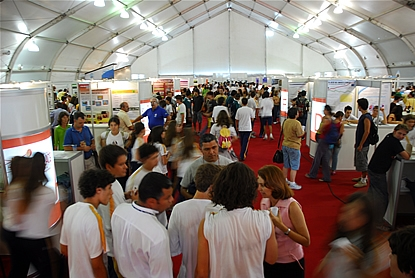
\includegraphics[width=1.0\linewidth]{arquivos/febrace.jpg}
        \end{center}
        \caption{Tenda da FEBRACE}
        \label{febrace}
    \end{figure}

A abrangência da FEBRACE pode ser vista através da tabela~\ref{abrangencia}. Segundo estatística da organização, no ano de 2009, houve a participação de 600 estudantes finalistas, 286 professores orientadores e 241 avaliadores, além de cerca de 30 voluntários. A feira foi visitada por cerca de 12 mil pessoas nos três dias de exposição. 

\begin{table}[h]
    \begin{center}
        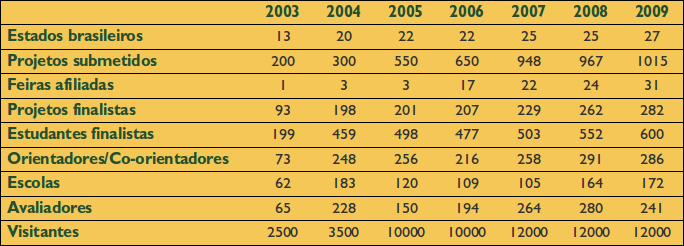
\includegraphics[width=0.8\linewidth]{arquivos/abrangencia.png}
    \end{center}
    \caption{FEBRACE em números}
    \label{abrangencia}
\end{table}

A feira conta com a participação de diversas pessoas com os papéis descritos abaixo:

\begin{description}
    \item[Finalistas] 
        são estudantes dos ensinos fundamental, médio e técnico com no máximo 25 anos que estão expondo seus projetos na feira;
    \item[Orientadores] 
        são pessoas com idade acima de 21 anos que orientaram os projetos expostos, podendo ser ou não professores;
    \item[Co-orientadores] 
        são pessoas com idade acima de 18 anos que ajudaram na orientação dos projetos expostos, podendo ser ou não professores e
    \item[Acompanhantes] 
        são outras pessoas que vêm junto com os alunos para acompanhá-los durante a feira, como familiares e diretores de escolas. Há também os estudantes observadores.
\end{description}

A FEBRACE não conta só com pessoas ligadas ao LSI para sua organização. Há uma equipe de apoio, formada em sua maioria por estudantes de graduação que disponibilizam de seu tempo para participar como voluntários. Entre suas atividades estão acompanhar os participantes em excursões culturais e científicas e apoio aos expositores na tenda. Para a avaliação dos projetos expostos, também existe uma equipe de avaliadores, que são pessoas com no mínimo mestrado em uma das áreas de interesse da feira.

A FEBRACE possui sete categorias, que são uma adaptação da tabela de áreas e sub-áreas do conhecimento adotada pela Fapesp (Fundação de Amparo à Pesquisa do Estado de São Paulo):

\begin{description}
    \item[Ciências Agrárias:] 
        Agronomia, Recursos Florestais e Engenharia Florestal, Engenharia Agrícola, Zootecnia, Medicina Veterinária, Recursos Pesqueiros e Engenharia de Pesca, Ciência e Tecnologia de Alimentos
    \item[Ciências Biológicas:] 
        Biologia Geral, Bioquímica, Genética, Biofísica, Botânica, Farmacologia, Zoologia, Imunologia, Ecologia, Microbiologia, Morfologia, Parasitologia, Fisiologia 	 
    \item[Ciências Exatas e da Terra:] 
        Matemática, Física, Probabilidade e Estatística, Química, Ciência da Computação, Geociências, Astronomia, Oceanografia 
    \item[Ciências Humanas:] 
        Filosofia, Geografia, Sociologia, Psicologia, Antropologia, Educação, Arqueologia, Ciência Política, História, Teologia 
    \item[Ciências da Saúde:] 
        Medicina, Odontologia, Fonoaudiologia, Farmácia, Enfermagem, Fisioterapia e Terapia Ocupacional, Nutrição, Saúde Coletiva, Educação Física
    \item[Ciências Sociais Aplicadas:] 
        Direito, Museologia, Administração, Comunicação, Economia, Serviço Social, Arquitetura e Urbanismo, Economia Doméstica, Planejamento Urbano e Regional, Desenho Industrial, Demografia, Turismo, Ciência da Informação  	 
    \item[Engenharias:] 
        Eletrônica, Sanitária, Eletrotécnica, de Produção, Mecânica, Nuclear, Química, de Transportes, Civil, Naval e Oceânica, de Minas, Aeroespacial, de Materiais e Metalúrgica, Biomédica 
\end{description}

A FEBRACE trabalha com o conceito de feiras afiliadas. Uma feira regional pode se afiliar e com isso pode enviar um certo número de projetos representantes que varia de acordo com seu tamanho e abrangência.

Além de sua importância nacional, a FEBRACE é uma feira afiliada à Intel ISEF (Intel International Science and Engineering Fair) realizada anualmente em maio em diferentes cidades dos Estados Unidos da América. A Intel ISEF é a maior feira de ciências do mundo voltada a estudantes dos ensinos fundamental e médio e o Brasil é uma das 50 nações participantes.

A discussão acima expõe o importante papel social da FEBRACE no estímulo à reflexão e à aprendizagem de forma criativa pelos estudantes da educação básica através do desenvolvimento de projetos de ciências e engenharia. Percebe-se que incentivos nesse sentido aos estudantes influenciam em seu interesse por uma formação técnica e/ou superior em alguma ciência e em seu espírito de inovação, estimulando avanços em termos tecnológicos e científicos para o país.

Apesar da importante função desempenhada pela FEBRACE, ela possui uma abrangência limitada para o tamanho do território brasileiro. Devido a limitações de espaço na tenda de eventos há uma necessidade de selecionar os projetos a serem expostos através de uma pré-avaliação. Muitos dos recusados possuem um bom nível e teriam condições para participar, mas não há como comportá-los. Além disso, a feira não possui verba para financiar a vinda dos participantes de outras cidades, sendo que eles devem cobrir os gastos de suas viagens e estadias em São Paulo. Sem patrocínio, alguns projetos aprovados não conseguem arcar com os custos de sua participação na feira.

A reunião de pessoas de todo o Brasil em um mesmo espaço físico, apesar da abrangência de oportunidades e experiências proporcionadas, é algo caro. Por outro lado, as Tecnologias da Informação e da Comunicação (TICs) oferecem muitas ferramentas que suprem as necessidades de interação entre as pessoas e um conjunto delas, os \textit{Softwares} Sociais, vêm crescendo muito nos últimos anos no mundo todo, tanto na gama de serviço disponíveis quanto na base de usuários conectados. Um \textit{Software} Social é aquele que permite a comunicação e interação ricas entre seus usuários. As formas de interação possibilitadas por esse tipo de aplicação são as mais diversas: adição de usuários como amigos, envio de mensagens entre usuários, comentário em postagem de \textit{blog} de outro usuário, discussão de um determinado assunto com outros usuários interessados, compartilhamento de vídeos, etc. Há diversos exemplos de \textit{Softwares} Sociais que podem ser citados como Orkut, Twitter e Facebook. Segundo \citeonline{futurelab06}, o desenvolvimento do \textit{Software} Social e as mudanças de objetivo na educação indicam estar indo para a mesma direção.

Nesse contexto, esse projeto de formatura alia as idéias de \textit{Software} Social e de Feira de Ciências, criando assim uma Feira Virtual de Ciências. 

Com o intuito de aumentar o alcance da feira, levando-a por mais tempo a mais pessoas e estimulando a criação de redes entre elas, foi criada uma aplicação de código fonte aberto que possibilita a exposição dos projetos na Internet e que oferece ferramentas para aumentar a interação entre os diversos envolvidos na Feira. Além disso, o envolvimento de pessoas em projetos e a troca de informações entre pessoas interessadas em feiras de ciências será facilitado, catalizando o papel social da FEBRACE.
